\section{Context Viewpoint}

\subsection{Stakeholder Model}
\begin{figure}[H]
    \centering
    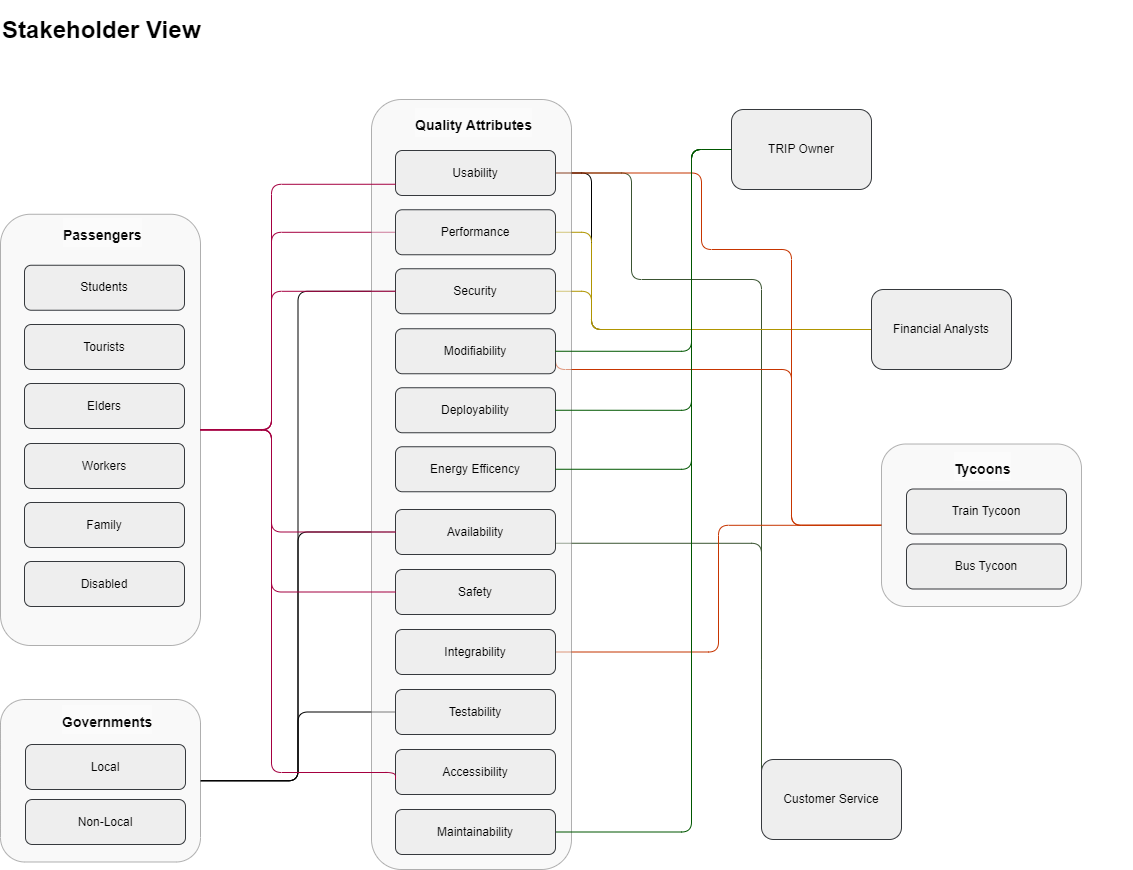
\includegraphics[width=\textwidth]{drawings/views_final_version/stakeholder_view.png}
    \caption{Stakeholder model of the TRIP system.}
    \label{fig:stakeholder_view_model}
\end{figure}

\subsection{Context Model}
\begin{figure}[H]
    \centering
    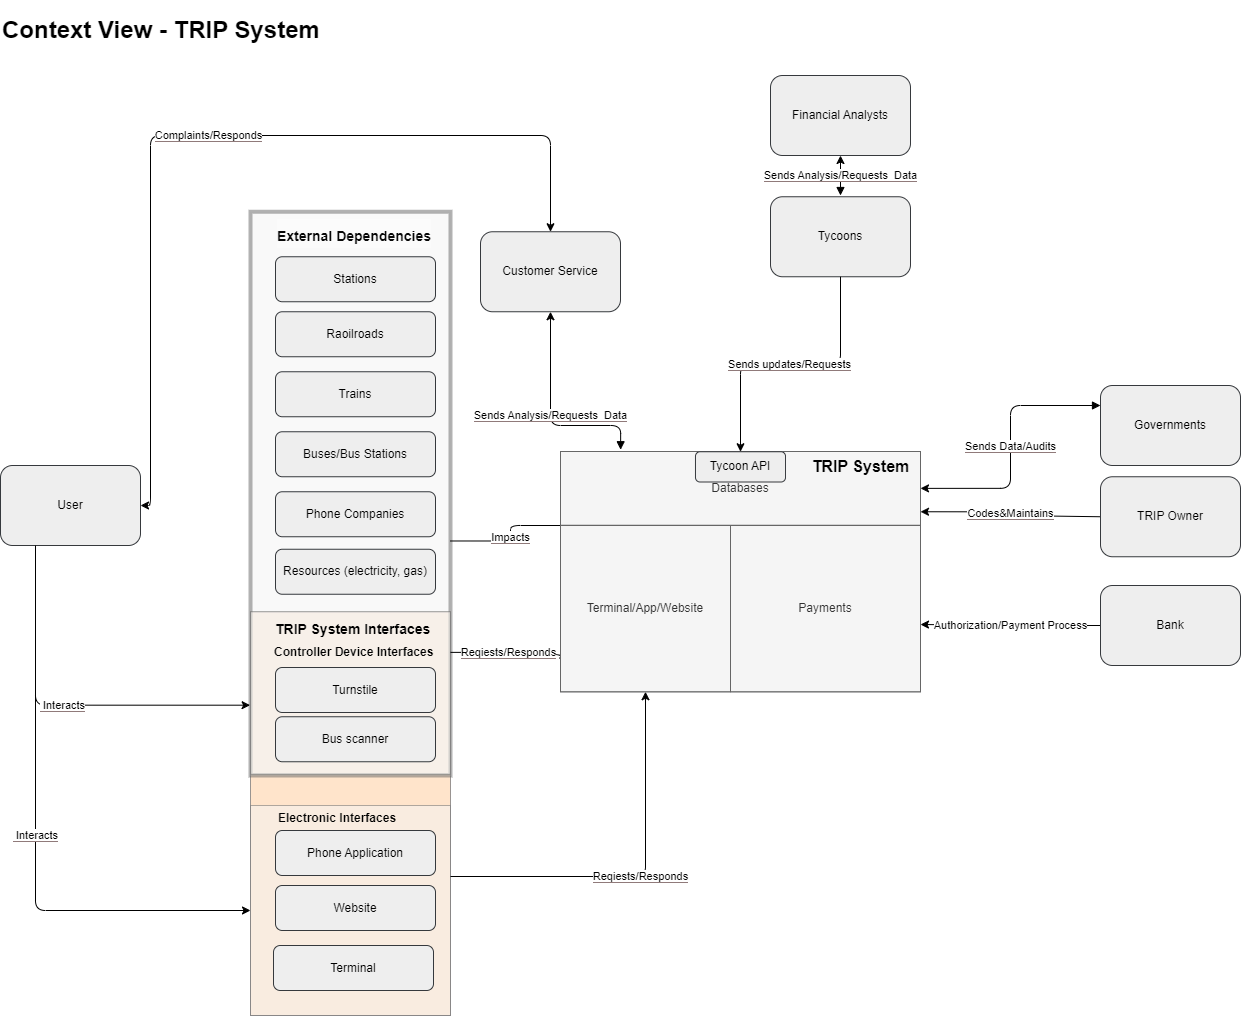
\includegraphics[width=\textwidth]{drawings/views_final_version/context_view.png}
    \caption{Context model of the TrIP system.}
    \label{fig:context_view_model}
\end{figure}

\subsection*{Description}
The Context View of the TRiP SYSTEM delineates the ecosystem within which the system operates, including its interactions with users, external entities, and other system components. At the user level, engagement with the TRiP system is facilitated through various interfaces such as terminals, apps, websites, and controller devices like turnstiles and bus scanners, enabling passengers to access services seamlessly.

The system is subject to a range of external dependencies, including infrastructure elements like stations, railroads, and trains, as well as service providers such as phone companies and utilities that supply essential resources. These components are integral to the system's operations, impacting its functionality and performance.

At the core, the TRiP system is interconnected with Tycoons via the Tycoon API, through which data flows bidirectionally, allowing for the exchange of updates, requests, and analytical data. The databases within the system are pivotal in managing schedules, user accounts, tickets, and payments, all of which are crucial for the day-to-day operations.

The system's architecture is designed to ensure robustness and responsiveness to both the passengers' and Tycoons' needs. It facilitates various processes, from payment transactions, which are securely handled and routed through financial institutions, to the maintenance of service quality, overseen by the TRiP owner and regulated by governmental audits and codes. This comprehensive network of interactions defines the TRiP system's context, emphasizing its multifaceted nature and the critical role it plays in serving its stakeholders.

\begin{table}[H]
\centering
\begin{tabular}{@{}clp{9cm}@{}}
\toprule
\textbf{Id} & \textbf{Name} & \textbf{Description} \\
\midrule
1 & Passenger & Individuals who use the TrIP SYSTEM and its associated services, interacting through various interfaces. \\
2 & Customer Service & The department that handles passenger complaints and feedback, providing support and sending analysis or data requests to the system. \\
3 & Financial Analysts & Experts or entities that review financial data, requiring analytical information from the system for decision-making. \\
4 & Tycoons & The operational decision-makers of the system, possibly managers or algorithms that control system parameters and require data. \\
5 & Tycoon API & The programming interface through which Tycoons receive updates and send requests to the system. \\
6 & TrIP System & The core system that integrates various interfaces and processes, forming the central operation platform. \\
7 & Governments & Regulatory bodies that may require data or perform audits on the system for governance and compliance. \\
8 & TrIP Owner & The entity or person owning and maintaining the TrIP SYSTEM, responsible for its overall functionality. \\
9 & Bank & Financial institution that handles the authorization and processing of payments for the system. \\
10 & Stations & Locations where the TrIP SYSTEM provides service to passengers, such as train or bus stations. \\
11 & Railroads & Infrastructure providers that offer the tracks on which train services operate. \\
12 & Trains & The vehicles used by the system to transport passengers from one station to another. \\
13 & Buses/Bus Stations & The bus services and their stations that are part of the transport network. \\
14 & Phone Companies & Telecom service providers that facilitate mobile communication and data transfer for the system. \\
15 & Resources (electricity, gas) & Utility providers that supply essential power and energy required for the system’s operations. \\
16 & Controller Device Interfaces & The interfaces like turnstiles and bus scanners that manage access control and validate user credentials. \\
17 & Electronic Interfaces & Digital platforms such as mobile applications and websites that passengers interact with for services. \\
\bottomrule
\end{tabular}
\caption{Context model glossary for the TrIP System.}
\label{tab:glossary_context_view}
\end{table}

\section{Functional Viewpoint}
\begin{figure}[H]
    \centering
    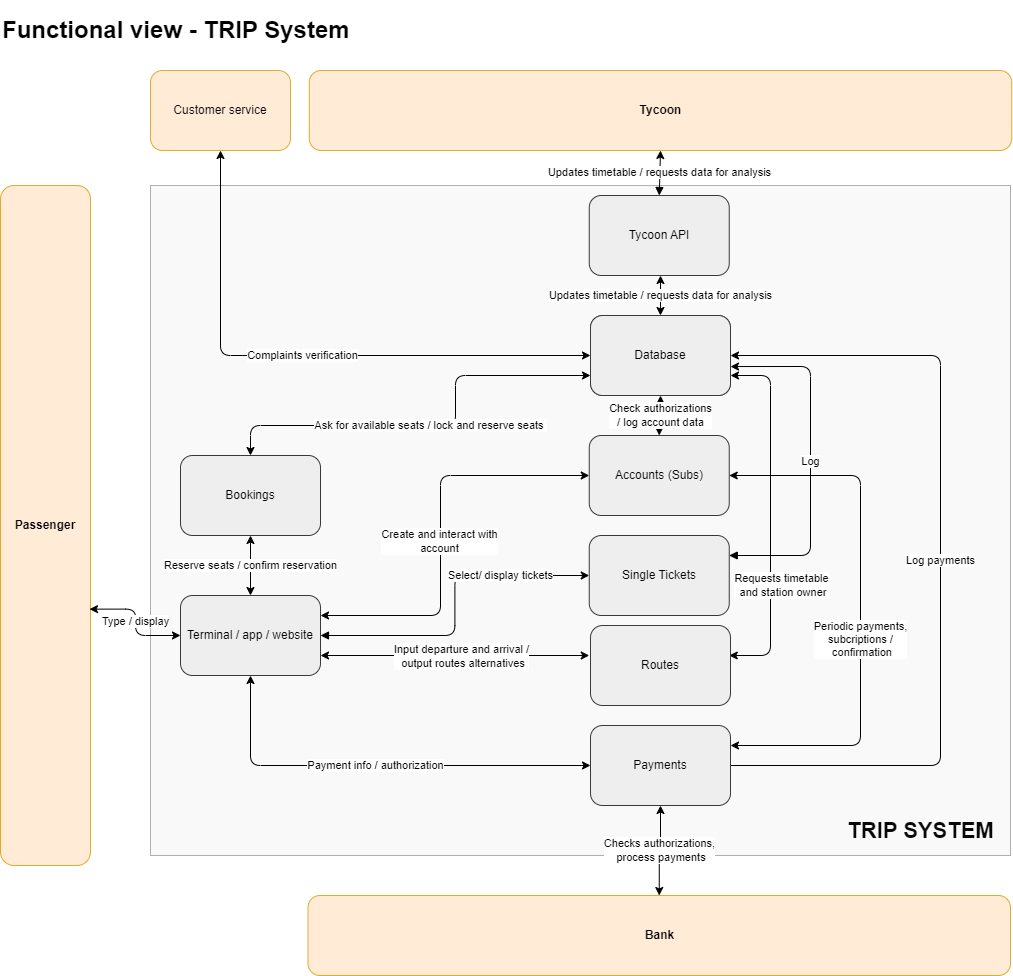
\includegraphics[width=\textwidth]{drawings/views_final_version/functional_view.png}
    \caption{TrIP System.}
    \label{fig:trip_system}
\end{figure}

\subsection*{Description}
The functional view diagram of the TrIP system illustrates the major functions of the system and how they interact with each other. The diagram features boxes representing different functions, connected by arrows that represent interactions.
The system starts with the user, who can interact with the system through various interfaces, such as terminals, apps, or websites. The user can input their departure and arrival stations, and the system will then display a list of available routes. The user can then select a route and proceed to payment.
The payment system can handle various payment methods, including single tickets, subscriptions, and fillable cards. If the user has a subscription, the system will automatically check if the subscription is valid for the selected route. This is done by the Account and Subscription Management module, which communicates with the tycoon systems to verify the subscription. If the subscription is not valid, the user will be prompted to purchase a single ticket or top up their fillable card.
Once the payment is processed, the system will generate a ticket or update the user's travel card. The user can then scan their ticket or card at the turnstile to gain access to the train platform. The turnstile communicates with the Account and Subscription Management module to verify the ticket or card and update the passenger's state.
The system also includes a number of other functions, such as a booking system, a route optimization system, and a customer service system. The booking system allows users to reserve seats on trains. The route optimization system helps users find the most efficient routes between their departure and arrival stations. The customer service system provides support to passengers with inquiries and complaints.
The system is designed to be scalable and flexible, so that it can be easily adapted to accommodate new tycoons and changing business models. The system is also designed to be secure, so that passenger data is protected from unauthorized access.

\begin{table}[H]
    \centering
    \begin{tabular}{@{}clp{9cm}@{}}
    \toprule
    \textbf{Id} & \textbf{Name} & \textbf{Description} \\
    \midrule
    1 & Passenger & End-users of the TrIP SYSTEM who interact with various system components to manage their travel experience. \\
    2 & Customer Service & The interface for passengers to make inquiries or complaints and receive assistance with bookings or account issues. \\
    3 & Tycoon & The administrative or business logic module that updates timetables and analyzes system data for improvements or reporting. \\
    4 & Database & An abstraction for the set of databases that stores all system data including passenger accounts, bookings, and payment information. Detailed information about how different databases are handled is detailed in the Information View.\\
    5 & Bookings & The system component where passengers can inquire about seat availability and make reservations. \\
    6 & Accounts (Subs) & The system managing passenger accounts and subscriptions, responsible for authorization checks and account data logging. 
    It is is also responsible for single tickets and fillable cards, as they can be seen as temporary and anonymous accounts. \\
    7 & Routes & The component that manages route information and provides passengers with timetables, station ownership details, and route alternatives. \\
    8 & Payments & The module handling all financial transactions, including passenger payments and periodic billing. \\
    9 & Bank & The financial institution interface for authorizing and processing payments linked to the system. \\
    10 & Terminal/App/Website & User interfaces through which they can access services such as booking, route information, and payment. \\
    \bottomrule
    \end{tabular}
    \caption{Glossary of elements detailing the components of the TrIP SYSTEM and their roles in facilitating user interaction and service provision.}
    \label{tab:glossary_trip_system}
\end{table}

\begin{figure}[H]
    \centering
    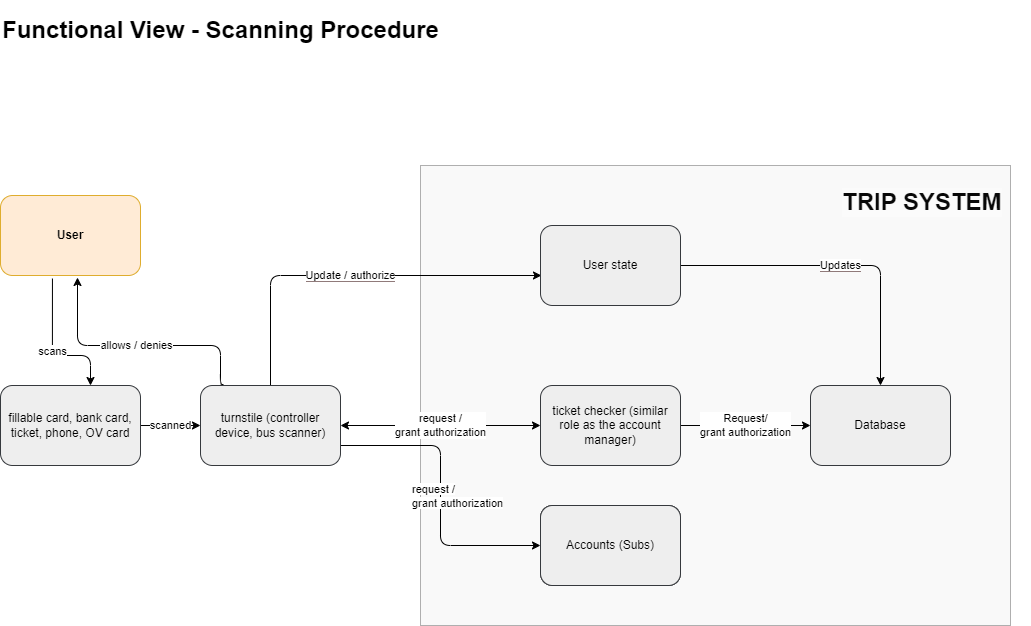
\includegraphics[width=\textwidth]{drawings/views_final_version/functional_view scanning.png}
    \caption{Interaction with a ticket scanner.}
    \label{fig:ticket_scanner}
\end{figure}

\subsection*{Description}
The scanning procedure within the TRIP SYSTEM encapsulates the interactions between the passenger and the system's access control mechanisms. It begins with the user presenting a valid form of transit access—such as a card or mobile device—to a scanning device like a turnstile or bus scanner. This device then consults the User state, a repository of the passenger's authorization status, to allow or deny entry. In parallel, the Ticket Checker function verifies the user's credentials against the Accounts subsystem, which manages detailed account information and subscriptions. Any changes to the user's status are updated in real time in the central Database, ensuring accurate tracking of access and travel history. This process ensures a secure, streamlined experience for passengers while providing the system with the necessary oversight to prevent unauthorized access

\begin{table}[H]
    \centering
    \begin{tabular}{@{}clp{9cm}@{}} % Adjust the width of the description column as needed to fit the page
    \toprule
    \textbf{Id} & \textbf{Name} & \textbf{Description} \\
    \midrule
    1 & Passenger & The individual who uses the trip system and interacts with various components such as turnstiles and ticket checkers. \\
    2 & Fillable Card, Bank Card, Ticket, Phone, OV Card & Various forms of identification or payment methods that the passenger can use within the system. These are scanned by the turnstile to allow or deny access. \\
    3 & Turnstile (Controller Device, Bus Scanner) & A physical barrier or scanner that reads the passenger's ticket or card and determines whether to grant or deny access based on the passenger state or account information. \\
    4 & Passenger State & A system component that maintains the current state of the passenger within the system, including authorization and access rights, which is updated upon passenger interaction with the turnstile. \\
    5 & Ticket Checker (Account Manager) & An agent or system role similar to the account manager that requests or grants authorization for passenger access, potentially by checking the passenger state against the database. \\
    6 & Accounts (Subs) & The subsystem managing passenger accounts and subscriptions, which may interact with the turnstile and ticket checker to verify and update passenger access rights. \\
    7 & Database & An abstraction for the set of databases that stores all system data including passenger accounts, bookings, and payment information. Detailed information about how different databases are handled is detailed in the Information View.\\
    \bottomrule
    \end{tabular}
    \caption{Glossary of elements for the Functional View - Turnstiles, detailing the components and their roles in passenger access and authorization within the TrIP SYSTEM.}
    \label{tab:glossary_turnstiles}
\end{table}

\subsection{Analysis on Perspectives}

\begin{table}[h!]
    \centering
    \resizebox{\textwidth}{!}{%
    \begin{tabular}{|l|c|c|c|c|c|c|c|c|c|}
      \hline
      & Usability & Performance & Security & Modifiability & Cost Efficiency & Availability & Safety & Integrability & Maintainability \\
      \hline
      Functional View & 
      \cellcolor{gray!60}X & % Usability (2nd priority)
      \cellcolor{gray!30}X & % Performance (3rd priority)
      & & 
      \cellcolor{gray!55}X & % Cost (3rd priority)
      \cellcolor{gray!15}X & % Availability (4th priority)
      & & 
      \cellcolor{gray!90}X \\ % Maintainability (1st priority)
      \hline
    \end{tabular}
    }
    \caption{Functional View Prioritized Quality Attributes}
    \label{tab:functional_view}
\end{table}

\subsubsection{Scenarios}
% Scenario 1: Usability Enhancement through Standardized UIs
\begin{table}[H]
    \centering
    \begin{tabularx}{\textwidth}{@{} lX @{}}
    \toprule
    \textbf{Aspect} & \textbf{Details} \\
    \midrule
    Source & Passenger interacts with the payment terminal UI. \\
    Stimulus & The passenger navigates the options to buy a ticket. \\
    Artifact & Standardized User Interface (UI) of the payment terminal. \\
    Response & The UI displays a clear, consistent, and intuitive navigation path for ticket purchase. \\
    Measure & 95\% of passengers successfully purchase tickets without assistance. \\
    \bottomrule
    \end{tabularx}
    \caption{Scenario for Usability - Standardized UIs}
    \label{table:usability_enhancement}
\end{table}


% Scenario 2: Scalability via Tycoon API
\begin{table}[H]
    \centering
    \begin{tabularx}{\textwidth}{@{} lX @{}}
    \toprule
    \textbf{Aspect} & \textbf{Details} \\
    \midrule
    Source & A new tycoon's system attempting to integrate with the TrIP system. \\
    Stimulus & The tycoon sends a request to access route and fare data. \\
    Artifact & Tycoon API that standardizes data exchange with the TrIP system. \\
    Response & The API facilitates the integration, providing access to the required data. \\
    Measure & Integration is completed within 3 business days, with zero errors in data format conversion. \\
    \bottomrule
    \end{tabularx}
    \caption{Scenario for Scalability via Tycoon API}
    \label{table:scalability_tycoon_api}
\end{table}

% Scenario: Payment Flexibility for Diverse User Groups
% Scenario: Accommodating Varied Payment Preferences
\begin{table}[H]
    \centering
    \begin{tabularx}{\textwidth}{@{} lX @{}}
    \toprule
    \textbf{Aspect} & \textbf{Details} \\
    \midrule
    Source & Passengers with varying preferences for payment, each approaching the transit system's access points. \\
    Stimulus & Passengers select their payment method of choice, ranging from physical cash for single rides to digitally managed subscriptions, and some opt for the convenience of pre-loaded fare cards. \\
    Artifact & Integrated payment and authentication platform within the TrIP system. \\
    Response & The system adeptly manages the assortment of transactions, crediting cash payments, verifying subscription validity, and debiting pre-loaded cards, all in a streamlined fashion. \\
    Measure & The system consistently processes transactions of all types with a rapid response rate, registering a less than 2-second average processing time and maintaining a transaction success rate of 99\%. \\
    \bottomrule
    \end{tabularx}
    \caption{Scenario for Usability via Accommodating Varied Payment Preferences}
    \label{table:varied_payment_preferences}
\end{table}

In addressing the Quality Attribute (QA) priorities highlighted by users, our functional viewpoint incorporates several key decisions designed to enhance usability, maintainability, scalability, and performance efficiency.

To meet the usability needs of users, we have opted for standardized User Interfaces (UIs). These UIs, being open-source and widely utilized, benefit from a large user base that contributes to their maintenance and robustness. This choice ensures a user-friendly and reliable interface for passengers over the long term. Furthermore, it aligns with the TrIP owner's preferences by offering ease of maintenance and low operational costs.

The introduction of multiple payment methods, including fillable cards, credit cards, and single tickets, significantly simplifies passenger interaction with the TrIP system. The integration of accounts and subscriptions further facilitates seamless travel across multiple tycoon networks, enabling passengers to efficiently manage and use their subscriptions.

In response to Event 1, which underscored the need for easier integration of new tycoons, we have implemented the Tycoon API. This API standardizes data requests from each tycoon, irrespective of their mode of transportation, thus facilitating the smooth integration of new tycoons into the system. The Tycoon API, in conjunction with the accounts and bookings module, ensures that passengers can effortlessly utilize their subscriptions across different networks and book their preferred routes.

Event 3, which focused on traffic jams, raised the importance of optimizing system performance during peak periods. By deciding on a centralized route management module, we have streamlined data flow between the TrIP system and the tycoons. This module not only simplifies data management but also enhances the system's ability to handle high request volumes through optimization and caching strategies.

In summary, the functional viewpoint of our system meticulously addresses the initial QA priorities, along with the challenges presented by new tycoon integration (Event 1) and traffic jams (Event 3). These decisions collectively ensure a user-friendly, scalable, and high-performing TrIP system for passengers, tycoons, and the TrIP owner alike.




\section{Information Viewpoint}

\begin{figure}[H]
    \centering
    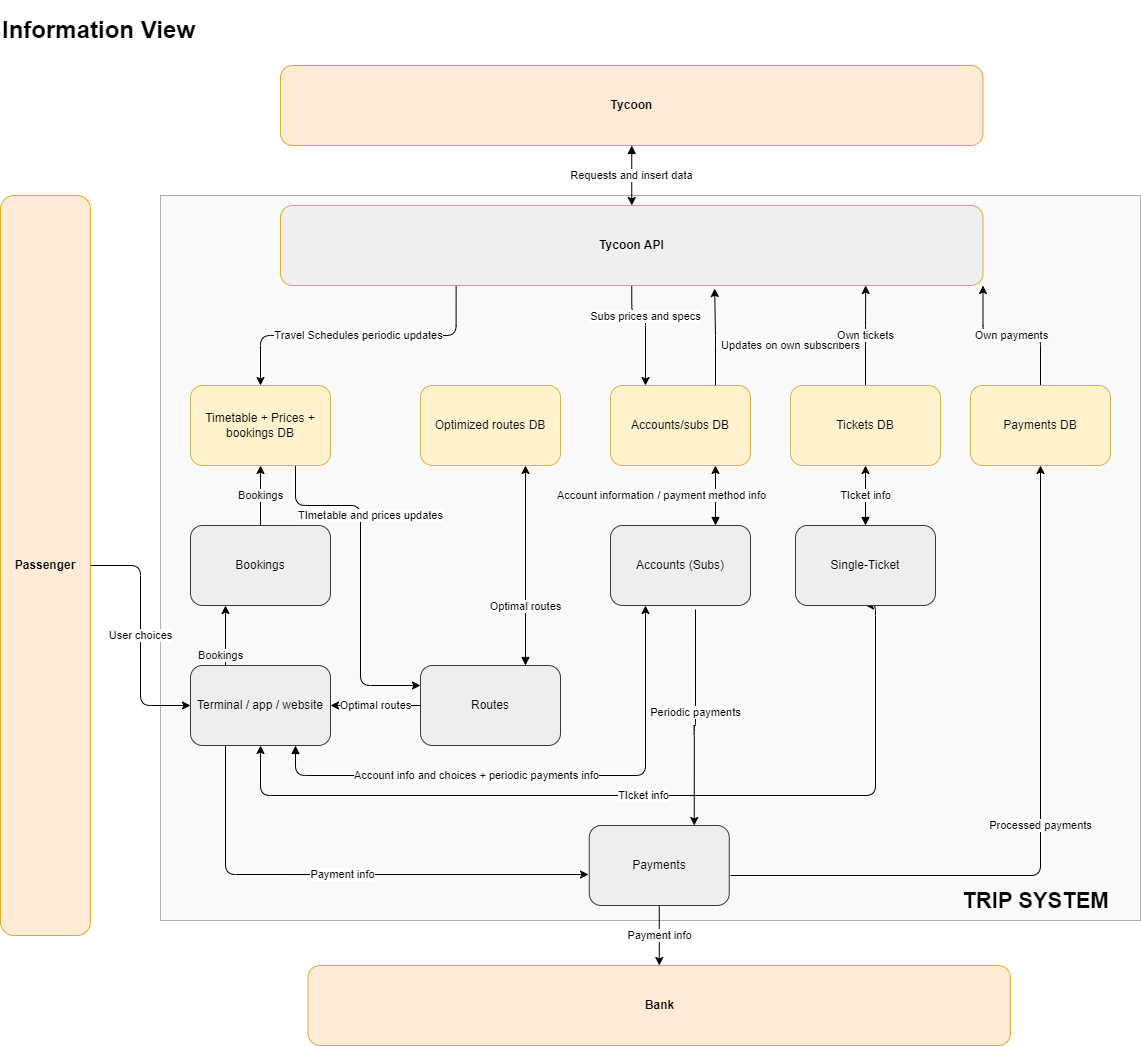
\includegraphics[width=\textwidth]{drawings/views_final_version/information_view.png}
    \caption{Information view.}
    \label{fig:information_view}
\end{figure}

\subsection*{Description}
The Information View of the TrIP SYSTEM is about how data moves and is stored. The system uses several databases. The Timetable + Prices + Bookings DB keeps track of schedules, prices, and reservations. The Optimized Routes DB has data on the best travel paths. The Accounts/Subs DB holds information on user accounts and subscriptions. The Tickets DB records ticket purchases, and the Payments DB keeps a record of all payments.

Tycoons use the Tycoon API to put in and get data. Passengers use terminals, apps, or websites to book travel and select routes. This choice and payment info go into the databases, updating the system.

The Routes component uses the Optimized Routes DB to give passengers the best travel options. The Accounts (Subs) part handles subscription details and payments, working with the Accounts/Subs DB. For single tickets, there's a separate interface that works with the Tickets DB. Payments process transactions and send completed payment information to the bank.

\begin{table}[H]
    \centering
    \caption{Glossary of elements for the Information View of the TrIP SYSTEM.}
    \label{tab:information_view_glossary}
    \begin{tabularx}{\textwidth}{@{}lX@{}} % Use 'X' for auto-adjusting width
    \toprule
    \textbf{Element} & \textbf{Description} \\
    \midrule
    Tycoon & Tycoons responsible for making requests for analysis, and inserting travel data. \\
    Tycoon API & Tycoon's way of interacting to the TrIP system. \\
    Timetable + Prices + bookings DB & Stores data regarding travel schedules, pricing, and booking information. \\
    Optimized routes DB & Contains information on the most efficient travel routes that have been calculated and stored. \\
    Accounts/Subs DB & Maintains records of user accounts and their subscriptions for travel services. \\
    Tickets DB & A database that logs ticket purchases and holds ticket-related information. \\
    Payments DB & Records and processes transactions related to payments within the system. \\
    Passenger & The end-user or customer who utilizes the system for travel services. \\
    Bookings & The system component or interface that passengers interact with to manage and view their bookings. \\
    Terminal / App / Website & The various platforms through which passengers can access the system for services. \\
    Routes & Involves the determination and selection of travel routes within the system. \\
    Accounts (Subs) & Manages the subscription details associated with user accounts. \\
    Single-Ticket & A system or interface that deals with the purchase of individual travel tickets. \\
    Periodic payments & Manages recurring payments, typically for subscription services. \\
    Payments & Processes transactions related to immediate payments within the system. \\
    Processed payments & A log or record of payment transactions that have been completed. \\
    Bank & The financial institution where final payment transactions are processed and funds are transferred. \\
    \bottomrule
    \end{tabularx}
\end{table}

\begin{figure}[H]
    \centering
    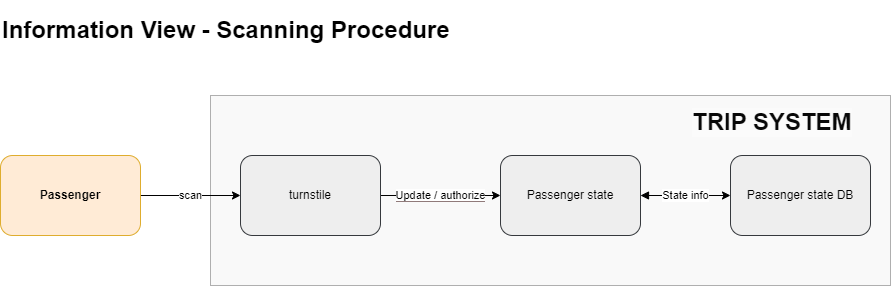
\includegraphics[width=\textwidth]{drawings/views_final_version/information_view scanning.png}
    \caption{Information view related to the scanning procedure.}
    \label{fig:information_view_scanning}
\end{figure}

\subsection*{Description}
The TrIP SYSTEM's scanning procedure is a sequence that starts with the Passenger, who scans at the Turnstile to gain entry. This triggers the Update/Authorize process, updating the Passenger State with the user's access rights. The Passenger State reflects the user's current permissions within the TRIP SYSTEM. Each user’s information is recorded in the Passenger State DB, a database that tracks and manages user statuses.

\begin{table}[H]
    \centering
    \caption{Legend for the Scanning Procedure in the Information View of the TrIP SYSTEM.}
    \label{tab:scanning_procedure_legend}
    \begin{tabular}{@{}llp{10cm}@{}}
    \toprule
    \textbf{Id} & \textbf{Name} & \textbf{Description} \\
    \midrule
    1 & Passenger & The starting point representing the individual using the TrIP SYSTEM. \\
    2 & Turnstile & The physical or virtual entry point where the passenger scans to gain access. \\
    3 & Update / Authorize & The process that updates the system and authorizes the passenger to proceed. \\
    4 & Passenger State & The current status of the passenger within the system, which is updated after scanning. \\
    5 & Passenger State DB & The database that records the state information of the passenger. \\
    \bottomrule
\end{tabular}
\end{table}

\subsection{Analysis on Perspectives}
\begin{table}[h!]
    \centering
    \resizebox{\textwidth}{!}{%
    \begin{tabular}{|l|c|c|c|c|c|c|c|c|c|}
      \hline
      & Usability & Performance & Security & Modifiability & Cost Efficiency & Availability & Safety & Integrability & Maintainability \\
      \hline
      Information View & 
       & % Usability
       & % Performance
      \cellcolor{gray!90}X & % Security (1st priority)
       & % Modifiability
       & % Cost Efficiency
       & % Availability
       & % Safety
       & % Integrability
       \\ % Maintainability
      \hline
    \end{tabular}
    }
    \caption{Information View Prioritized Quality Attributes}
    \label{tab:information_view}
\end{table}

\subsubsection{Scenarios}
% Scenario: Protecting Passenger Personal and Travel Information
\newcommand{\scenarioOneInformation}{
\begin{table}[H]
    \centering
    \begin{tabularx}{\textwidth}{@{} lX @{}}
    \toprule
    \textbf{Aspect} & \textbf{Details} \\
    \midrule
    Source & Passenger utilizing the TrIP system to manage their travel plans. \\
    Stimulus & The passenger enters personal and travel data into the system. \\
    Artifact & Encrypted Account Lookup Database within the TrIP system. \\
    Response & The system securely stores the passenger's data using state-of-the-art encryption both at rest and in transit, ensuring that personal and travel information is not accessible by unauthorized entities. Access to this data is restricted to specific operations within the TrIP system that require passenger verification. \\
    Measure & Passenger data breaches are non-existent, and passengers report a high level of trust in the system's data protection capabilities. Security logs show no unauthorized access, affirming the integrity of the encryption measures. \\
    \bottomrule
    \end{tabularx}
    \caption{Scenario for Security - Passenger Data Protection}
    \label{table:passenger_data_security}
\end{table}
}

% Scenario: Secure Payment Processing for Passenger Transactions
\newcommand{\scenarioTwoInformation}{
\begin{table}[H]
    \centering
    \begin{tabularx}{\textwidth}{@{} lX @{}}
    \toprule
    \textbf{Aspect} & \textbf{Details} \\
    \midrule
    Source & Passenger making a payment through the TrIP system. \\
    Stimulus & The passenger chooses a payment method and initiates a transaction. \\
    Artifact & Bank interfaced with TrIP system for processing payments. \\
    Response & The bank processes the payment with rigorous security protocols, ensuring that the payment information is handled in a secure, encrypted channel. The system guarantees that payment data is never stored within the TrIP system and is managed exclusively by the bank, providing an additional layer of security. \\
    Measure & Payment transactions are completed with zero incidents of data compromise, and the response time for transaction completion remains within 3 seconds. Post-transaction audits confirm the absence of payment data retention within the TrIP system. \\
    \bottomrule
    \end{tabularx}
    \caption{Scenario for Security - Secure Payment Transactions}
    \label{table:payment_transaction_security}
\end{table}
}

% Scenario: Controlled Access to Passenger Account Data
\newcommand{\scenarioThreeInformation}{
\begin{table}[H]
    \centering
    \begin{tabularx}{\textwidth}{@{} lX @{}}
    \toprule
    \textbf{Aspect} & \textbf{Details} \\
    \midrule
    Source & Passenger subscribing to a specific tycoon's services within the TrIP system. \\
    Stimulus & The subscribed tycoon requests access to the passenger's account data for service personalization. \\
    Artifact & Tycoon API enabling access control to passenger data within the TrIP system. \\
    Response & The TrIP system authenticates the tycoon's request through the Tycoon API, which validates that only the tycoon with whom the passenger is subscribed can retrieve the required data. This ensures that each tycoon can access only their passengers’ data, thus maintaining strict data access control and privacy. \\
    Measure & Regular audits indicate 100\% compliance with data access policies, with no reported incidents of data leakage or unauthorized access. Passenger feedback confirms trust in the data privacy practices of the TrIP system. \\
    \bottomrule
    \end{tabularx}
    \caption{Scenario for Security - Controlled Tycoon Access to Passenger Data}
    \label{table:tycoon_access_control}
\end{table}
}

The Information View of the TrIP system provides a comprehensive architecture designed to handle and safeguard data movement and storage, ensuring the system's integrity and security.

The design segregates data across specialized databases, including those for Timetables + Prices + Bookings, Optimized Routes, Accounts/Subs, Tickets, and Payments. This segregation follows best practices in database security, preventing any single point of compromise and ensuring each database only holds data relevant to its function. Access to these databases is strictly regulated, with the system enforcing robust authentication and authorization mechanisms to verify and control interactions.

Encryption plays an important role in the system, particularly within the Accounts/Subs Database. It protects sensitive passenger information by using encrypted account lookup database. Data at rest within this database, as well as data in transit to and from it, is encrypted, thereby securing personal and travel information from unauthorized access.

Payments are a critical interaction point for the system and its users. The TrIP system approaches this by interfacing directly with banks for payment processing. This interface means that the sensitive financial information is managed within the secure domain of banking institutions, which are inherently designed to handle such data securely. This direct interfacing also implies that the TrIP system does not store payment details, which greatly reduces its liability and exposure to financial data breaches.

The Tycoon API serves as a broker for data access by tycoons. It provides a controlled access point, permitting only authorized tycoons to retrieve passenger data. This access control mechanism is crucial for maintaining passenger privacy and data security. It allows tycoons to access only the data necessary for their service offerings and nothing beyond that.

Using the scenarios provided, we can see how the system's design and technology choices map directly to its operations. Passengers entering their information into terminals or apps can be assured that their data will be encrypted and stored securely, as detailed in the first scenario. Payment processes, as per the second scenario, happen within the secure confines of the banking system. Lastly, the way the Tycoon API manages data requests ensures that passenger data is only accessed by authorized tycoons, enhancing privacy and data protection as outlined in the third scenario.

\section{Concurrency Viewpoint}

\begin{figure}[H]
    \centering
    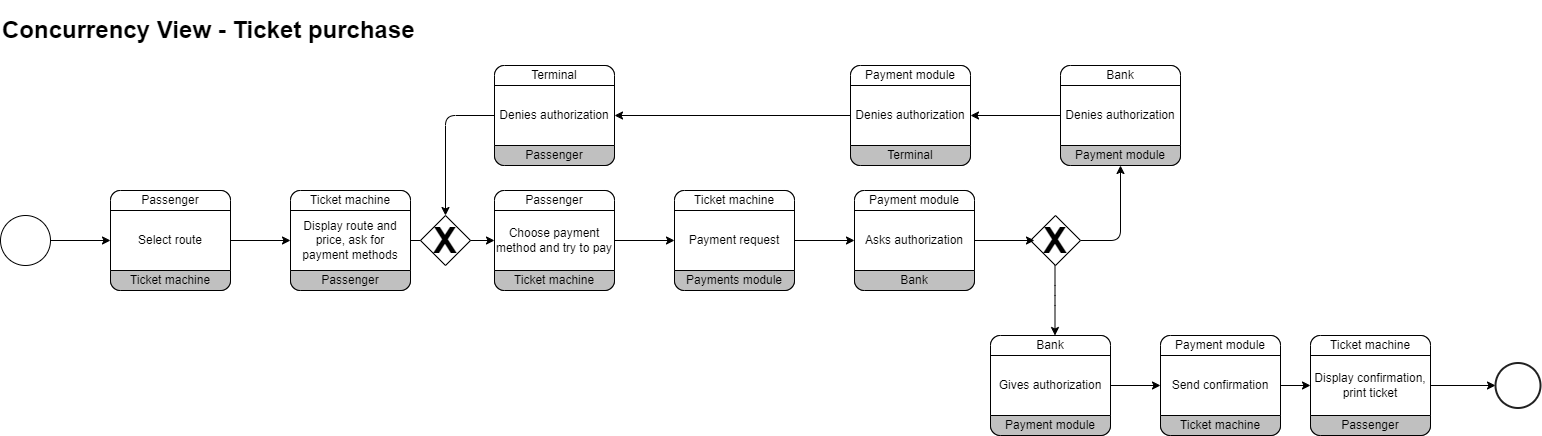
\includegraphics[width=\textwidth]{drawings/views_final_version/concurrency_view_1.png}
    \caption{Concurrency view related to ticket purchase.}
    \label{fig:concurrency_view_1}
\end{figure}

\subsection*{Description}
In the TRIP SYSTEM, the Passenger starts the process at the Ticket Machine, choosing a route and payment method. The Terminal takes over to process the payment, and the Payment Module communicates with the Bank for payment approval. If the Bank approves, the Payment Module signals the Ticket Machine to confirm the transaction and print the ticket. If the Bank denies the payment, the process is stopped, and the Passenger is notified.

\begin{table}[H]
    \centering
    \caption{Glossary for the Payment and Ticketing Process.}
    \label{tab:payment_ticketing_glossary}
    \begin{tabularx}{\textwidth}{@{}lX@{}} % Use 'X' for auto-adjusting width
    \toprule
    \textbf{Element} & \textbf{Description} \\
    \midrule
    Passenger & The customer who initiates the process by selecting a route and choosing a payment method to pay for a ticket. \\
    Ticket Machine & The interface through which the passenger selects a route, displays the route and price, and chooses a payment method. \\
    Terminal & The point of service where the passenger's payment authorization is processed. \\
    Payment Module & The system component that interacts with the bank to request payment authorization for the transaction. \\
    Bank & The financial institution that either authorizes or denies the payment transaction. \\
    \bottomrule
    \end{tabularx}
\end{table}

\begin{figure}[H]
    \centering
    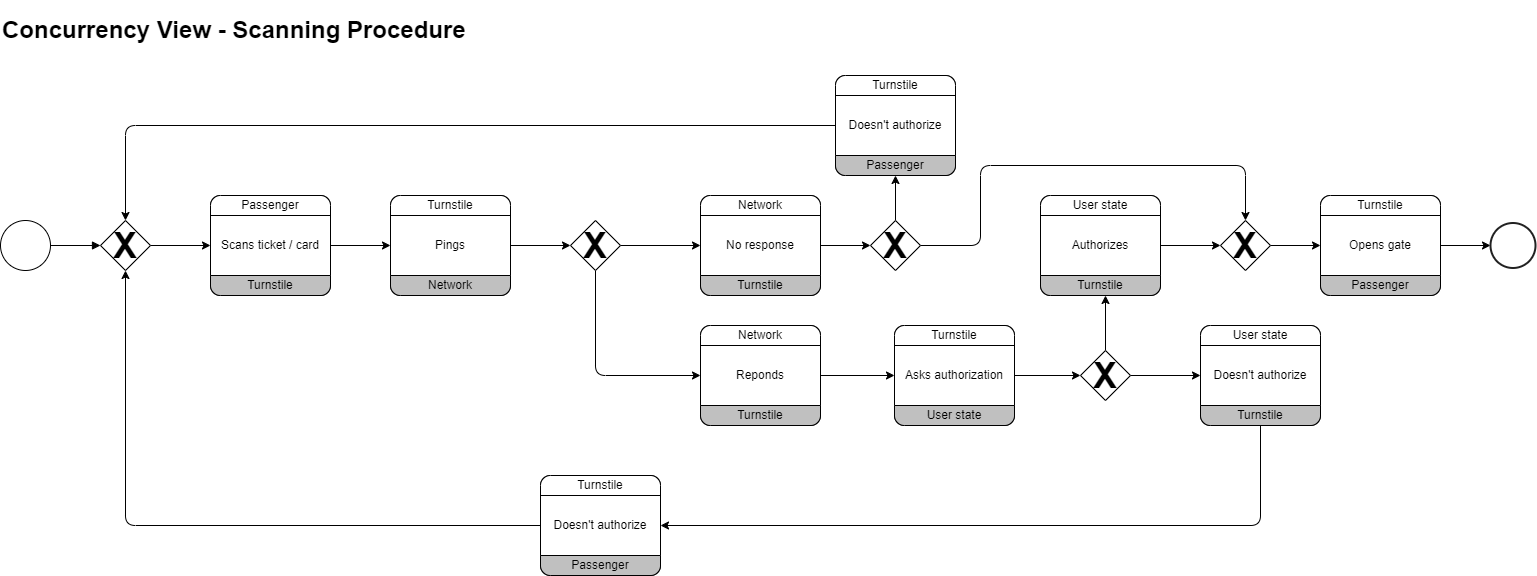
\includegraphics[width=\textwidth]{drawings/views_final_version/concurrency_view_2.png}
    \caption{Concurrency view related to the scanning procedure.}
    \label{fig:concurrency_view_2}
\end{figure}

\subsection*{Description}
The diagram depicts a turnstile access procedure with conditional paths based on network availability and user authorization. When a Passenger scans their ticket or card at the Turnstile, two scenarios can unfold:

\begin{enumerate}
    \item If the Turnstile is unable to connect to the Network (no response), it defaults to a local decision. In this case, the turnstile can still potentially authorize the passenger to proceed based on offline data or preconfigured rules.
    \item If the Turnstile connects to the Network (network responds), it then requests authorization from the User State. The User State, after evaluating the request, either grants or denies authorization:
    \begin{itemize}
        \item If the User State authorizes the request, the Turnstile receives a signal to open the gate, allowing the Passenger to pass.
        \item If the User State denies the request, the Turnstile will not open, and the Passenger is not allowed to proceed.
    \end{itemize}
\end{enumerate}

This process ensures that the system can function and provide decisions autonomously, even in the absence of network connectivity, enhancing reliability and user experience.

\begin{table}[H]
    \centering
    \caption{Glossary for Turnstile Interaction Process.}
    \label{tab:turnstile_interaction_glossary}
    \begin{tabularx}{\textwidth}{@{}lX@{}} % Use 'X' for auto-adjusting width
    \toprule
    \textbf{Component} & \textbf{Description} \\
    \midrule
    Passenger & An individual who is attempting to gain entry through the turnstile by scanning a ticket or card. \\
    Turnstile & A physical barrier at an entry point that controls access, typically based on ticket or card validation. \\
    Network & The communication system that the turnstile interfaces with to verify access rights. \\
    User State & A system component that maintains the current state of a user's access rights, determining whether entry is authorized. \\
    \bottomrule
    \end{tabularx}
\end{table}

\begin{figure}[H]
    \centering
    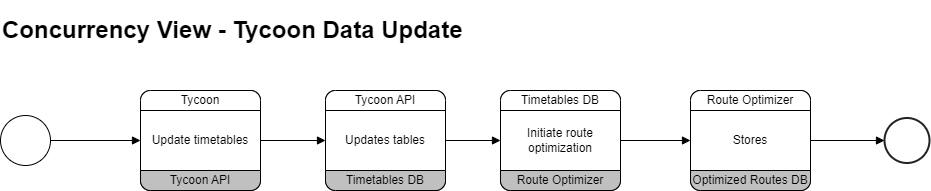
\includegraphics[width=\textwidth]{drawings/views_final_version/concurrency_view_3.png}
    \caption{Concurrency view related to tycoons data updates.}
    \label{fig:concurrency_view_3}
\end{figure}

\subsection*{Description}
This process outlines how timetable updates and route optimization are handled in the system. It begins with the Tycoon, an administrative role, who updates timetables through the Tycoon API. These updates are then applied to the Timetables DB. Following this update, the Route Optimizer initiates the optimization process, which takes the updated timetable data to determine the most efficient routes. These optimized routes are then stored in the Optimized Routes DB, completing the cycle of updating and optimizing the route information available to the system and its users.

\begin{table}[H]
    \centering
    \caption{Glossary for Route Optimization Process.}
    \label{tab:route_optimization_glossary}
    \begin{tabularx}{\textwidth}{@{}lX@{}} % Use 'X' for auto-adjusting width
    \toprule
    \textbf{Component} & \textbf{Description} \\
    \midrule
    Tycoon & Represents the train companies or transport entities responsible for managing train schedules and routes. \\
    Tycoon API & The application programming interface that allows the tycoons to update and access timetable information. \\
    Timetables DB & The database where train schedules, routes, and associated data are stored and updated. \\
    Route Optimizer & The system component that calculates the most efficient routes, likely using algorithms to process timetable data. \\
    Optimized Routes DB & A specialized database that stores the results of the route optimization process. \\
    \bottomrule
    \end{tabularx}
\end{table}

\subsection{Analysis on Perspectives}
\begin{table}[h!]
    \centering
    \resizebox{\textwidth}{!}{%
    \begin{tabular}{|l|c|c|c|c|c|c|c|c|c|}
      \hline
      & Usability & Performance & Security & Modifiability & Cost Efficiency & Availability & Safety & Integrability & Maintainability \\
      \hline
      Concurrency View & 
       & % Usability
      \cellcolor{gray!30}X & % Performance (2nd priority)
       & % Security
       & % Modifiability
       & % Cost Efficiency
      \cellcolor{gray!90}X & % Availability (1st priority)
      \cellcolor{gray!60}X & % Safety
       & % Integrability
       \\ % Maintainability
      \hline
    \end{tabular}
    }
    \caption{Concurrency View Prioritized Quality Attributes}
    \label{tab:concurrency_view}
\end{table}

\subsubsection{Scenarios}
% Scenario: Ensuring Service Availability During Network Outages
\newcommand{\scenarioOneConcurrency}{
\begin{table}[H]
    \centering
    \begin{tabularx}{\textwidth}{@{} lX @{}}
    \toprule
    \textbf{Aspect} & \textbf{Details} \\
    \midrule
    Source & Network outage impacting the TrIP system's connectivity. \\
    Stimulus & A passenger attempts to validate their ticket at a turnstile during the outage. \\
    Artifact & Hybrid approach of delayed processing and local caching implemented in the TrIP system. \\
    Response & The turnstile, equipped with local caching, validates the passenger's ticket against stored data, allowing entry. Transaction details are queued for delayed processing once network connectivity resumes, ensuring no service disruption. \\
    Measure & Passenger service continuity is maintained with 99.9\% uptime, and ticket validations during outages show no significant delay, ensuring high system availability. \\
    \bottomrule
    \end{tabularx}
    \caption{Scenario for Availability - Network Outage Handling}
    \label{table:availability_network_outage}
\end{table}
}
% Scenario: Maintaining Safety through Authorized Access

\newcommand{\scenarioTwoConcurrency}{
\begin{table}[H]
    \centering
    \begin{tabularx}{\textwidth}{@{} lX @{}}
    \toprule
    \textbf{Aspect} & \textbf{Details} \\
    \midrule
    Source & TrIP system's safety protocols for access control. \\
    Stimulus & An individual attempts to access the transit system without a valid ticket or permission. \\
    Artifact & Turnstile with integrated validation system that checks for valid tickets. \\
    Response & The turnstile denies entry to the individual without a valid ticket, preventing unauthorized access and maintaining the safety and security of the transit environment. \\
    Measure & Zero reported incidents of unauthorized access, ensuring the safety of the transit system and its users. \\
    \bottomrule
    \end{tabularx}
    \caption{Scenario for Safety - Authorized Access Enforcement}
    \label{table:safety_authorized_access}
\end{table}
}

% Scenario: Optimizing Performance with Pre-stored Routes
\newcommand{\scenarioThreeConcurrency}{
\begin{table}[H]
    \centering
    \begin{tabularx}{\textwidth}{@{} lX @{}}
    \toprule
    \textbf{Aspect} & \textbf{Details} \\
    \midrule
    Source & Passenger requests the best route options via the TrIP system during peak hours. \\
    Stimulus & High demand for route information causes potential strain on the system. \\
    Artifact & Optimized Routes Database that stores frequently requested route data. \\
    Response & The TrIP system quickly retrieves optimized route options from the pre-stored data, providing the passenger with fast and efficient service without needing to compute the routes in real-time. \\
    Measure & The response time for route information requests during peak periods remains under 2 seconds, enhancing the overall performance of the system. \\
    \bottomrule
    \end{tabularx}
    \caption{Scenario for Performance - Efficient Route Retrieval}
    \label{table:performance_route_optimization}
\end{table}
}

The Concurrency Viewpoint is central to the TRiP system's architecture, focusing on ensuring that user interactions with the system occur smoothly and without delay, even when multiple operations are executed simultaneously. This viewpoint addresses the system's capacity to manage concurrent actions effectively, with a particular emphasis on maintaining performance, safety, and availability. \\

\noindent\textbf{Ticket Purchasing Process:} \\
The sequence begins with the passenger selecting a route and payment method via the Ticket Machine. This process is crucial for performance, as it demands a fast and seamless operation to prevent queues and delays. Once the payment method is chosen, the Terminal communicates with the Payment Module to process the transaction. The Payment Module's role here is two-fold: to ensure the safety of the transaction by validating payment with the bank and to maintain the system's performance by providing quick feedback to the Terminal. If the bank authorizes the payment, the Payment Module prompts the Ticket Machine to dispense a ticket, showcasing the system's availability to complete transactions without delay. In case of a denial, the passenger is promptly informed, allowing them to take alternative actions, which is vital for maintaining system usability and ensuring the passenger's experience remains positive. \\

\noindent \textbf{Turnstile Access Control:} \\
The second aspect of concurrency comes into play at the turnstiles, where passengers scan their tickets or cards to gain access to the transport services. In this operation, the system's availability and safety are the primary concerns. The Turnstile must quickly authorize entry to avoid creating bottlenecks, which it does by pinging the Network to retrieve the User State information. If the Network is unresponsive, the Turnstile uses locally cached data to make an authorization decision, ensuring continuous operation and thus maintaining high availability. When the Network responds, the User State determines access permission. This dual approach ensures that access control is robust against network issues, preserving the integrity of operations and passenger safety by preventing unauthorized access. \\

\noindent \textbf{Route Optimization Updates:} \\
Finally, the system’s capacity to update and optimize routes through the Tycoon API and Route Optimizer reflects its modifiability and performance attributes. Tycoons can update timetables, which are then processed to optimize routes, and these optimizations are stored in the Optimized Routes DB for quick retrieval. This ensures that passengers receive up-to-date and efficient routing information, which is especially important during peak traffic conditions. \\

By detailing these processes, the concurrency viewpoint showcases the TrIP system's capability to maintain a high level of service and security across its operations, aligning with the defined quality attributes of performance, safety, and availability.

\section{Deployment Viewpoint}

\begin{figure}[H]
    \centering
    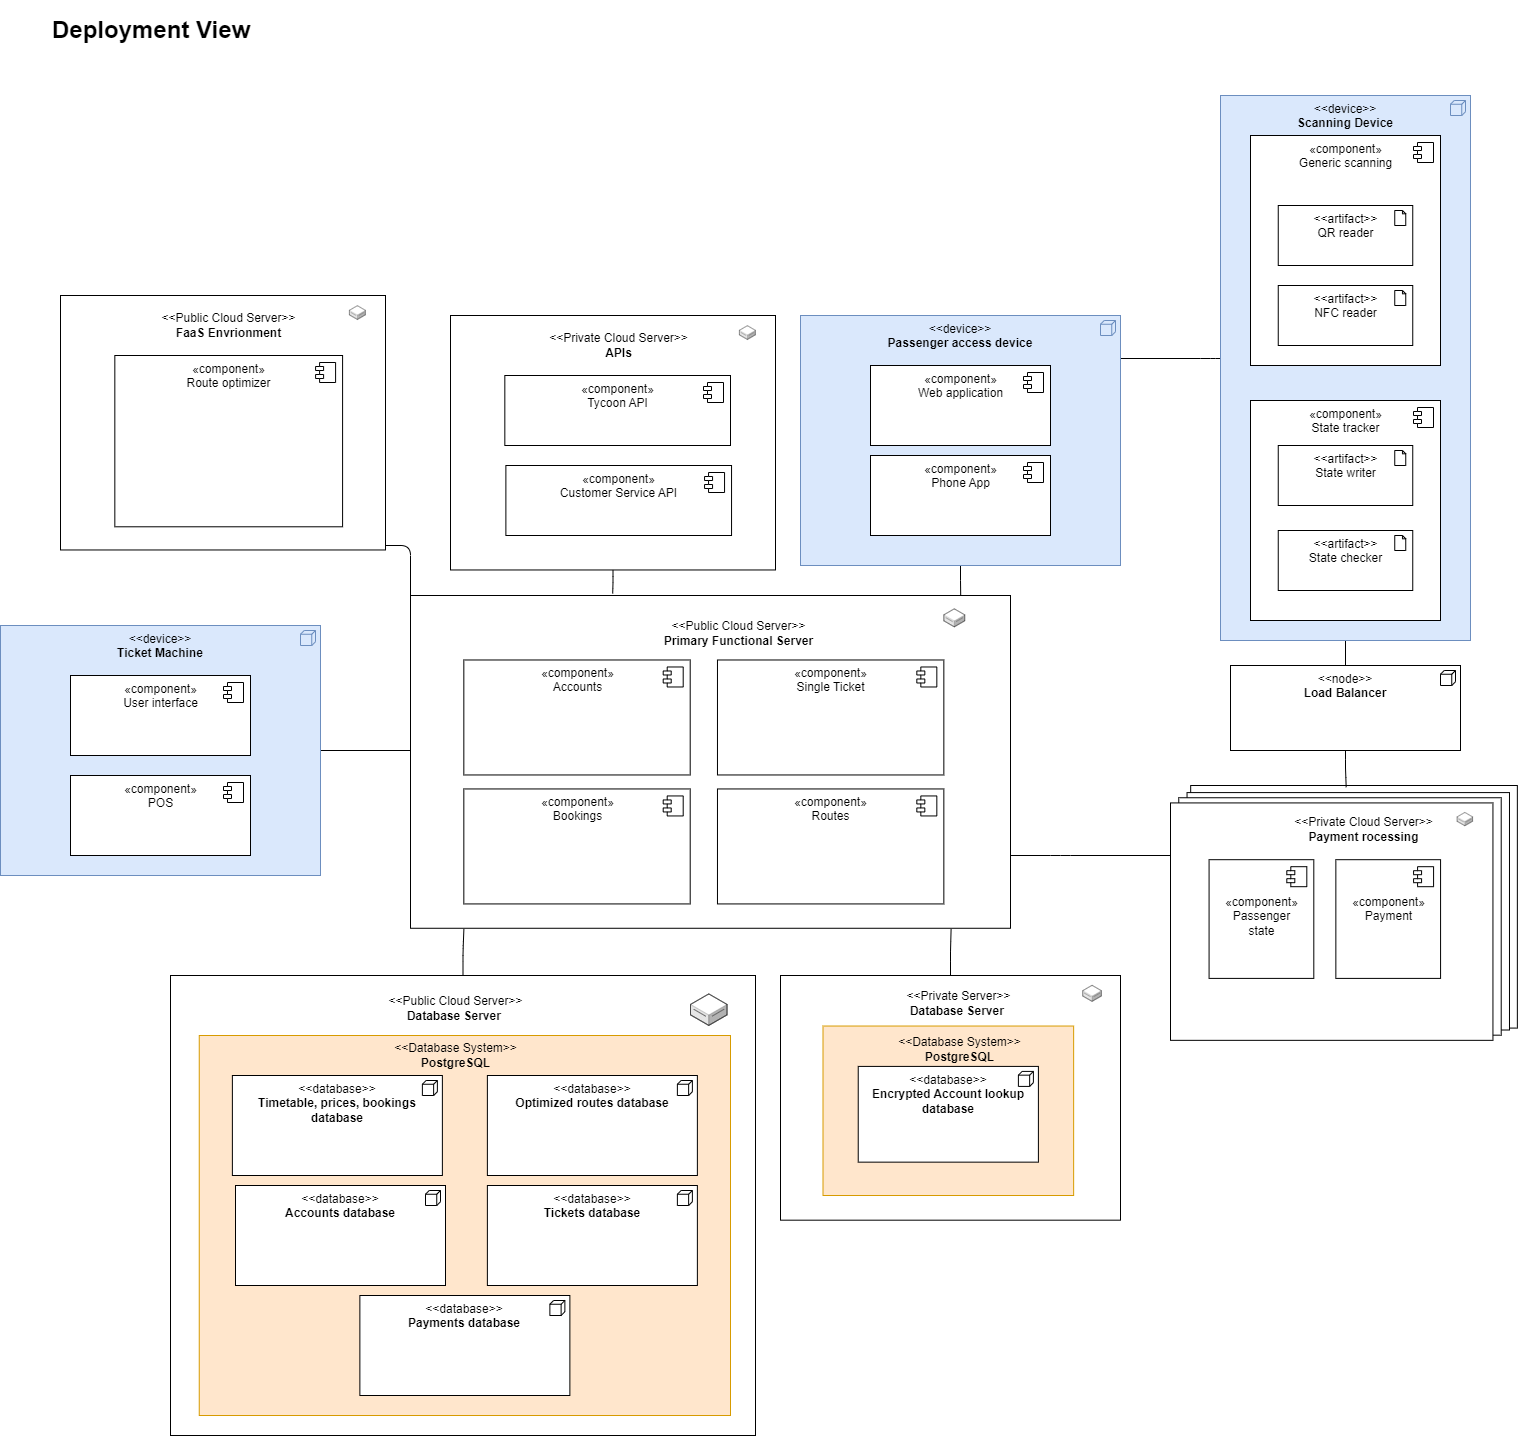
\includegraphics[width=\textwidth]{drawings/views_final_version/deployment_view.png}
    \caption{Deployment view related to the scanning procedure.}
    \label{fig:deployment_view_scanning}
\end{figure}

\subsection*{Description}
The deployment view diagram illustrates the TrIP system's architecture, showing components distributed across public and private cloud servers. Public cloud servers house the FaaS Environment for route optimization, a Terminal with Customer Service API, and the Primary Functional Server hosting Accounts, Single Ticket, Bookings, and Routes components. Devices for passenger access, such as web and phone apps, interface with scanning devices like QR and NFC readers, managed by state trackers and checkers.

The ticket machine interfaces include User Interface and POS components. Database servers in the public cloud manage the PostgreSQL databases for Timetables, Prices, Bookings, Optimized Routes, Accounts, Tickets, and Payments. The private cloud server secures the Encrypted Account Lookup database. A Load Balancer ensures efficient traffic management.

Payment processing, crucial for managing Passenger State and payments, is securely handled in the private cloud, emphasizing the system's focus on security and reliable transaction handling. 


\begin{table}[H]
    \centering
    \caption{Glossary for the Deployment View of the TrIP SYSTEM.}
    \label{tab:deployment_view_glossary}
    \begin{tabularx}{\textwidth}{@{}lXX@{}} % Corrected to have three columns
    \toprule
    \textbf{Component} & \textbf{Description} & \textbf{Hosted On} \\
    \midrule
    FaaS Environment & Provides a platform for executing backend functions in a serverless architecture, such as route optimization. & Public Cloud Servers \\
    Tycoon API & Interfaces allowing tycoons' software and systems to communicate with the TrIP system. & Private Cloud Servers \\
    Customer Service API & Facilitates customer service operations by providing data access and manipulation capabilities. & Private Cloud Servers \\
    Passenger Access Device & Equipment that passengers interact with to access the system, like ticket validation and purchases. & Terminal, App, Website \\
    Ticket Machine & Physical machines where passengers can purchase tickets and manage their bookings. & Station Locations \\
    Scanning Device & Tools used for reading ticket information, necessary for entry validation and passenger tracking. & Entry/Exit Gates \\
    QR Reader & Specialized scanners that interpret QR codes on tickets for entry validation or information retrieval. & Scanning Devices \\
    NFC Reader & Contactless devices that read NFC tags for authentication and ticket validation. & Passenger Access Devices \\
    Timetable, Prices, Bookings Database & Stores all relevant data for scheduling, pricing, and passenger bookings. & Public Cloud Servers \\
    Optimized Routes Database & Contains data on the most efficient routes calculated by the optimization algorithms. & Public Cloud Servers \\
    Accounts Database & Manages passenger account information, including subscription details and personal data. & Public Cloud Servers \\
    Tickets Database & Holds data related to ticket sales, validations, and historical transactions. & Public Cloud Servers \\
    Payments Database & Processes and records all payment transactions within the system. & Public Cloud Servers \\
    Encrypted Account Lookup Database & A secure database that stores sensitive account information, accessible only through authorized queries. & Private Cloud Servers \\
    \bottomrule
    \end{tabularx}
\end{table}

\subsection{Analysis on Perspectives}
\begin{table}[h!]
    \centering
    \resizebox{\textwidth}{!}{%
    \begin{tabular}{|l|c|c|c|c|c|c|c|c|c|}
      \hline
      & Usability & Performance & Security & Modifiability & Cost Efficiency & Availability & Safety & Integrability & Maintainability \\
      \hline
      Deployment View & 
       & % Usability
      \cellcolor{gray!90}X & % Performance (1st priority)
      \cellcolor{gray!60}X & % Security (3rd priority)
       & % Modifiability
       & % Cost Efficiency
       & % Availability (2nd priority)
       & % Safety
       & % Integrability
       \\ % Maintainability
      \hline
    \end{tabular}
    }
    \caption{Deployment View Prioritized Quality Attributes}
    \label{tab:deployment_view}
\end{table}

\subsubsection{Scenarios}
% Scenario: Upgrading Cloud Infrastructure for High Demand
\begin{table}[H]
    \centering
    \begin{tabularx}{\textwidth}{@{} lX @{}}
    \toprule
    \textbf{Aspect} & \textbf{Details} \\
    \midrule
    Source & TrIP system experiencing a surge in demand due to a new university opening at a station. \\
    Stimulus & Passenger numbers have more than quadrupled, causing performance delays during rush hours. \\
    Artifact & The deployment of the TrIP system across public cloud servers and private cloud servers. \\
    Response & The system's cloud infrastructure is updated to leverage elastic scaling capabilities. Load balancers distribute the increased traffic efficiently, and additional computing resources are allocated to handle the high load, particularly for route optimization and payment processing components. \\
    Measure & Post-update, the TrIP system handles a fourfold increase in user load with response times reduced by 70\%, ensuring that all passengers complete their transactions and receive route information within 2 seconds, even during peak rush hours. \\
    \bottomrule
    \end{tabularx}
    \caption{Scenario for Performance - Cloud Infrastructure Scaling}
    \label{table:performance_scaling}
\end{table}

% Scenario: Reinforcement of Data Security and Privacy Protocols
\begin{table}[H]
    \centering
    \begin{tabularx}{\textwidth}{@{} lX @{}}
    \toprule
    \textbf{Aspect} & \textbf{Details} \\
    \midrule
    Source & TrIP system architecture analysis in response to a competitor's security breach. \\
    Stimulus & The need to verify and bolster the security measures in place to protect passenger data. \\
    Artifact & Deployment architecture of the TrIP system with a focus on data servers and encryption protocols. \\
    Response & The system utilizes advanced encryption for data at rest and in transit within private cloud servers. Access controls are strictly enforced, ensuring only authenticated and authorized components interact with sensitive data. Periodic security audits and real-time intrusion detection systems are in place to monitor and immediately respond to any unauthorized access attempts. \\
    Measure & Security tests confirm no data leakage, and the system's compliance with the latest privacy regulations is validated by a third-party security firm, ensuring that the board and tycoons have verifiable assurance of the system's security measures. \\
    \bottomrule
    \end{tabularx}
    \caption{Scenario for Security - Privacy and Data Protection}
    \label{table:security_privacy}
\end{table}


In the Deployment Viewpoint, the TRiP system's architecture is strategically distributed across a combination of cloud-based and localized servers to optimize for both performance and security, critical attributes for the robustness and reliability of the system.

The TRiP system's deployment on cloud servers is engineered to enhance performance. The public cloud servers provide a scalable Fast Environment for handling dynamic user demands and instantaneous Route Optimization, ensuring that the most efficient paths are always available to the user. This optimization is further supported by Load Balancers, which are essential in managing network traffic by distributing workloads evenly, thereby preventing any server from becoming a bottleneck and ensuring a smooth user experience. 

For security, the system employs private cloud servers, where sensitive components such as the Encrypted Account Lookup Database are hosted. The encryption of this database is a crucial security measure, safeguarding personal and travel data against unauthorized access. 

Through this architecture, the TRiP system ensures the system is able handle the performance requirements from its users, while keeping the user information secure. Usage of cloud servers ensures dynamically scalable performance requirements. Keeping the state of the users, and caching optimzied routes is another architectural decision where the system is able to respond user requests fast with the scanning devices.

\section{Development Viewpoint}

\begin{figure}[H]
    \centering
    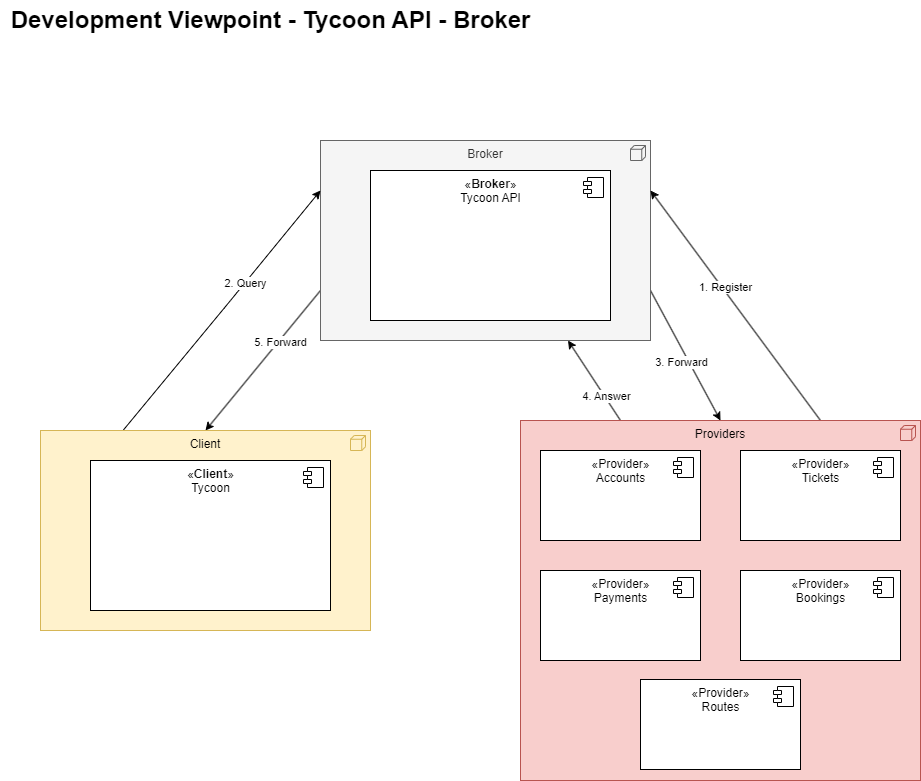
\includegraphics[width=\textwidth]{drawings/views_final_version/development_view_broker.png}
    \caption{Deployment view related broker pattern related to Tycoon API.}
    \label{fig:development_view_broker}
\end{figure}

\subsection*{Description}
The diagram portrays the broker architecture in the TrIP system, delineating the communication between clients, the broker, and providers. Tycoon clients initiate the interaction by registering with the Tycoon API broker. Queries are sent from the Tycoon to the broker, which then forwards these queries to the relevant providers. These providers include services for Accounts, Payments, Bookings, Tickets, and Routes, each playing a pivotal role in processing Tycoon requests. Upon gathering the necessary data or performing the required actions, providers send their response back to the broker. The broker, in turn, forwards this information back to the Tycoon client, completing the request-response cycle. This broker pattern facilitates a structured approach to handling requests and centralizes the communication logic, simplifying interactions across the system’s diverse components.


\begin{table}[H]
    \centering
    \caption{Glossary for the Broker in the Development View.}
    \label{tab:broker_development_glossary}
    \begin{tabular}{@{}llp{10cm}@{}}
        \toprule
    \textbf{Id} & \textbf{Name} & \textbf{Description} \\
    \midrule
    1 & Client & Represents the Tycoon requesting data or action from the broker. \\
    2 & Broker & Tycoon API that mediates between clients (Tycoon's) and various service providers (TrIP System's modules), handling requests and responses. \\
    3 & Provider & TrIP system that register with the broker to offer their services to clients. \\
    4 & Tycoon API & The application programming interface provided by the broker for communication with clients and providers. \\
    5 & Query & A request sent from the client to the broker, seeking information or action. \\
    6 & Register & The action of a provider adding their services to the broker's list of available resources. \\
    7 & Forward & The process of the broker sending requests to providers or responses back to clients. \\
    8 & Answer & The provider's response to a query that is sent back to the client via the broker. \\
    9 & Accounts & TrIP System module that manages user account information and authentication. \\
    10 & Tickets & TrIP system for issuing tickets, usually related to events or transportation. \\
    11 & Payments & The TrIP module that handles transaction processing. \\
    12 & Bookings & TrIP System module that manages reservations for services offered by the provider. \\
    13 & Routes & TrIP System module that handles route pricing. \\
    \bottomrule
    \end{tabular}
\end{table}


\begin{figure}[H]
    \centering
    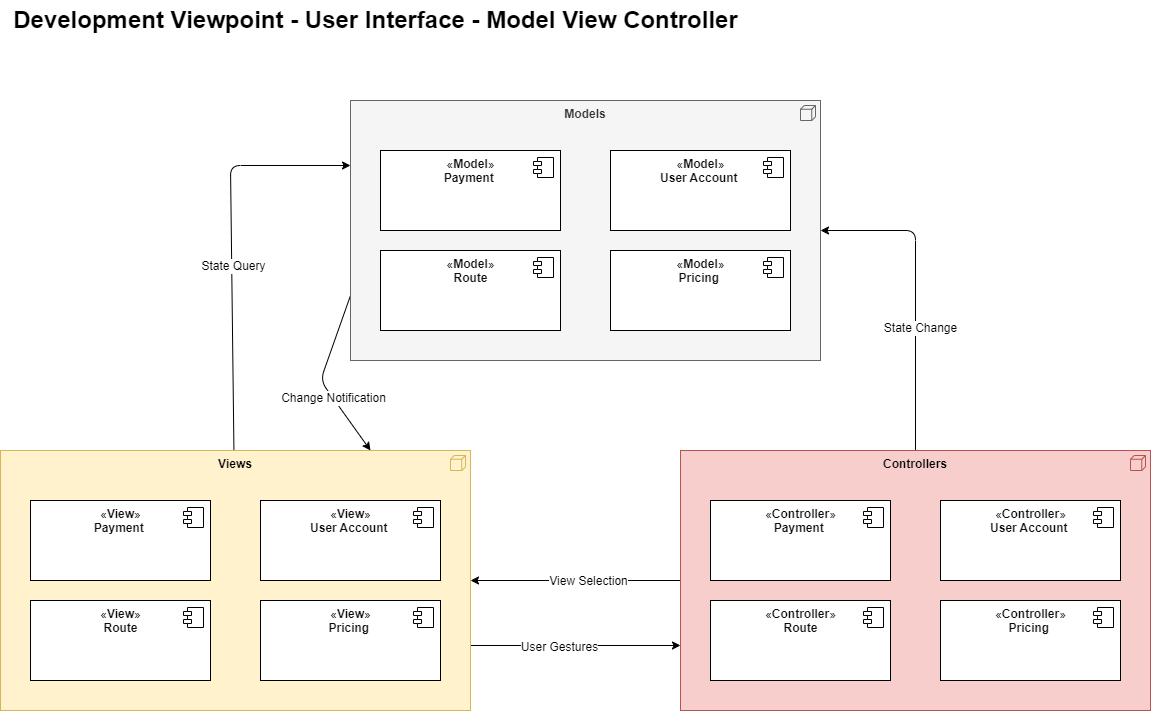
\includegraphics[width=\textwidth]{drawings/views_final_version/development_view_User_Interface.png}
    \caption{Development view model-view-controller pattern for UI}
    \label{fig:development_view_User_Interface}
\end{figure}

\subsection*{Description}
This diagram illustrates the Model-View-Controller (MVC) pattern applied within the TrIP system. It breaks down the system's user interface into Views, which are responsible for presenting data to users and include interfaces for Payment, User Account, Route, and Pricing. The Models act as the data layer with Payment, Route, User Account, and Pricing components that manage the system's state. They receive state queries and broadcast state changes to the Views. Controllers interpret user gestures, direct state changes, and mediate between the Models and Views. This separation of concerns ensures that user interactions are handled efficiently, system data is managed cohesively, and business logic is executed in a controlled manner. The MVC architecture is fundamental to the system's organization, promoting clear delineations between different functionalities and facilitating ease of maintenance and scalability.

\begin{table}[H]
    \centering
    \caption{Legend for the User Interface Components in the Development View of the TrIP System.}
    \label{tab:trip_system_ui_development_legend}
    \begin{tabular}{@{}llp{10cm}@{}}
    \toprule
    \textbf{Id} & \textbf{Name} & \textbf{Description} \\
    \midrule
    1 & Views & User interface components of the TrIP system that passengers interact with, including elements like payment, account management, and route selection screens. \\
    2 & Models & Data structures in the TrIP system that encapsulate the core business logic related to payment, user accounts, route information, and pricing. \\
    3 & Controllers & Components within the TrIP system that manage input from passengers, process requests, and produce responses by interacting with Models and updating Views. \\
    4 & Payment View/Model/Controller & Dedicated interfaces, data, and logic for processing passenger payments within the TrIP system, ensuring secure transactions. \\
    5 & User Account View/Model/Controller & Elements responsible for managing passenger profiles, including authentication and handling of personal account details in the TrIP system. \\
    6 & Route View/Model/Controller & Components that handle the presentation, data management, and operational logic of travel routes available to passengers in the TrIP system. \\
    7 & Pricing View/Model/Controller & The set of user interfaces, algorithms, and data that determine and manage fare calculations and display pricing information to passengers. \\
    8 & State Query & A request by the TrIP system to retrieve the current state, such as checking a passenger's account status or ticket validity. \\
    9 & State Change & An update within the TrIP system that alters the current state in response to passenger actions or other operational changes. \\
    10 & Change Notification & A notification mechanism that informs the TrIP system and passengers when a significant change has occurred, such as a payment confirmation or route update. \\
    11 & User Gestures & Interactions by passengers with the TrIP system, like touch or click actions, which are interpreted as commands to navigate or provide input. \\
    12 & View Selection & The process within the TrIP system for choosing the appropriate user interface view to display to passengers based on the current context or request. \\
    \bottomrule
    \end{tabular}
\end{table}

\subsection{Analysis on Perspectives}
\begin{table}[h!]
    \centering
    \resizebox{\textwidth}{!}{%
    \begin{tabular}{|l|c|c|c|c|c|c|c|c|c|}
      \hline
      & Usability & Performance & Security & Modifiability & Cost Efficiency & Availability & Safety & Integrability & Maintainability \\
      \hline
      Development View & 
      \cellcolor{gray!60}X & % Usability (2nd priority)
       & % Performance
       & % Security
       \cellcolor{gray!40}X& % Modifiability
       & % Cost Efficiency
       & % Availability
       & % Safety
       \cellcolor{gray!25}X& % Integrability
      \cellcolor{gray!90}X \\ % Maintainability (1st priority)
      \hline
    \end{tabular}
    }
    \caption{Development View Prioritized Quality Attributes}
    \label{tab:development_view}
\end{table}


\subsubsection{Scenarios}
% Scenario 1: Usability Enhancement through Standardized UIs
% Scenario: Efficient Data Retrieval for Tycoon Route Analysis and Account Information
\begin{table}[H]
    \centering
    \begin{tabularx}{\textwidth}{@{} lX @{}}
    \toprule
    \textbf{Aspect} & \textbf{Details} \\
    \midrule
    Source & Tycoon's analytical system requesting data for route pricing and passenger account details. \\
    Stimulus & The Tycoon system sends a data request to analyze route prices based on their subscription models and to gather specific account information for passengers. \\
    Artifact & Tycoon API interfacing between the Tycoon's systems and the TrIP system's databases. \\
    Response & The Tycoon API promptly routes the queries to the appropriate data providers, retrieves the requested information, and consolidates the results for the Tycoon system. \\
    Measure & Tycoon system receives comprehensive data within 3 seconds, enabling effective route and subscription analysis for passenger accounts. \\
    \bottomrule
    \end{tabularx}
    \caption{Scenario for Tycoon API Data Retrieval}
    \label{table:tycoon_api_data_retrieval}
\end{table}

% Scenario: Streamlined System Updates through MVC Pattern
\begin{table}[H]
    \centering
    \begin{tabularx}{\textwidth}{@{} lX @{}}
    \toprule
    \textbf{Aspect} & \textbf{Details} \\
    \midrule
    Source & TrIP system development team. \\
    Stimulus & The need to update the route pricing algorithm without affecting the user interface. \\
    Artifact & Model-View-Controller (MVC) pattern within the TrIP system. \\
    Response & Developers update the Pricing Model with the new algorithm, which automatically propagates changes to the relevant Views without requiring additional adjustments. \\
    Measure & The system update is deployed with zero downtime, and subsequent feature updates require 40\% less time due to decoupled architecture. \\
    \bottomrule
    \end{tabularx}
    \caption{Scenario for Maintainability - MVC Pattern}
    \label{table:mvc_maintainability}
\end{table}

% Scenario: Enhanced User Experience with MVC-Driven UI
\begin{table}[H]
    \centering
    \begin{tabularx}{\textwidth}{@{} lX @{}}
    \toprule
    \textbf{Aspect} & \textbf{Details} \\
    \midrule
    Source & Passenger using the TrIP system to manage travel. \\
    Stimulus & The passenger updates their travel preferences in the User Account View. \\
    Artifact & MVC pattern facilitating the User Account management. \\
    Response & The Controller processes the passenger's input, updates the User Account Model, and the View dynamically reflects the changes, providing immediate visual confirmation to the passenger. \\
    Measure & Passengers express a 90\% satisfaction rate with the ease of updating preferences, and the error rate in preference updates decreases by 50\%. \\
    \bottomrule
    \end{tabularx}
    \caption{Scenario for Usability - MVC-Driven UI}
    \label{table:mvc_usability}
\end{table}

The Development Viewpoint focuses on the structural aspects that underpin the TrIP system's architecture, highlighting the modular approach in system design to enhance usability and maintainability. \\

\noindent \textbf{MVC Pattern:} \\
The adoption of the Model-View-Controller (MVC) pattern substantially improves the system's maintainability by segregating the user interface elements (Views) from the business logic (Models) and user input processing (Controllers). This separation of concerns allows developers to update or modify one aspect of the system — such as adding new features to the user interface — without the need to alter the underlying business logic or control flow. For passengers, this results in a more comprehensive interface with a variety of options and features, enhancing the overall usability of the system. The MVC pattern ensures that as passenger needs evolve, new Views can be added swiftly, making the system both adaptable and future-proof. \\

\noindent \textbf{Broker Architecture:} \\
In parallel, the broker architecture employed within the Tycoon API streamlines the interaction process between the Tycoons and the TrIP system. It serves as a centralized point for processing queries and handling communications, thus simplifying the complexity of these interactions. For the Tycoons, this architecture means usability is significantly enhanced, allowing them to communicate through a unified interface with the Tycoon API, which abstracts the intricate workings of the TrIP system's service modules. This consolidation of communication logic not only benefits the Tycoons but also reduces the overhead for the TrIP system in managing multiple communication protocols. \\

These architectural decisions, reflected in the Development Viewpoint, are key to the TrIP system's ability to offer an efficient, secure, and user-friendly platform that can grow and adapt in line with technological advancements and user expectations.
